% = = = = = = = = = = = = = = = = = = = = = %
%           Concept Generation              %
% = = = = = = = = = = = = = = = = = = = = = %

\let\clearpage\relax
\chapter{Concept Generation}

\section{ISA} %sj
An instruction set architecture (ISA) describes the capabilities of a processor. The ISA specifies how instructions should be formatted so that the control unit can correctly interpret them, and the meaning of those instructions in terms of their semantics.

Besides, an ISA also defines the supported data types, the registers, the hardware support for managing main memory, fundamental features and the input/output model of a processor. As such, an ISA represents an interface between programmer and an abstract processor rather than an exact specification of how the processor should be implemented \cite{Daniel}.

Therefore, to design our personal processor, we must choose an ISA that satisfies our design requirement. A good ISA can help us achieve our design specifications easily.

An ISA may be classified in a number of different ways. A common classification is by architectural complexity. A complex instruction set computer (CISC) has many specialized instructions, some of which may only be rarely used in practical programs. A reduced instruction set computer (RISC) simplifies the processor by efficiently implementing only the instructions that are frequently used in programs, while the less common operations are implemented as subroutines, having their resulting additional processor execution time offset by infrequent use \cite{risc_cisc}.

We will make our decision among all these ISAs.

\section{Microarchitecture} %sl
Comparing to ISA, which describes the overall architecture of a computer system that is usually visible to programmers, microarchitecture usually describes the way that how a specific processor design implements the ISA. Namely, to some extent the concepts of ISA and microarchitecure are orthogonal, i.e., one ISA can be implemented by many processors, while one microarchitecture can support different ISAs after necessary modifications. Unlike ISA, usually microarchitecture is invisible to programmers. For instance, in our out-of-order microarchitecture design, although the instructions are dynamically scheduled and executed, from the perspective of programmer, the instructions seem to be executed sequentially and follow the programmers' intention.

Therefore, a good microarchitecture design is key to a successful processor product. Even though different processors share the same ISA, they may differ in microarchitecture designed for different kind of market, e.g., high-performance computing or embedded systems.

In terms of the number of instructions that can be executed at the same time, we have scalar design and superscalar design. Fig.~\ref{fig:superscalar} demonstrates the difference between two kinds of design. While scalar design is able to execute one instruction at a time, superscalar design supports multiple channels to execute the instructions. Theoretically, for example, a 2-way superscalar design can double the performance. However, in reality, due to many external factors, e.g., data and control dependency, the speed-up ratio should be between 1 and 2.

\begin{figure}[!htp]
    \centering
    \begin{subfigure}{0.4\textwidth}
      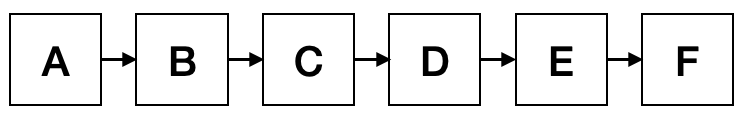
\includegraphics[width=\textwidth]{figure/scalar.png}
      \caption{Scalar execution.}
      \label{fig:superscalar-1}
  \end{subfigure}
  ~
  \begin{subfigure}{0.4\textwidth}
      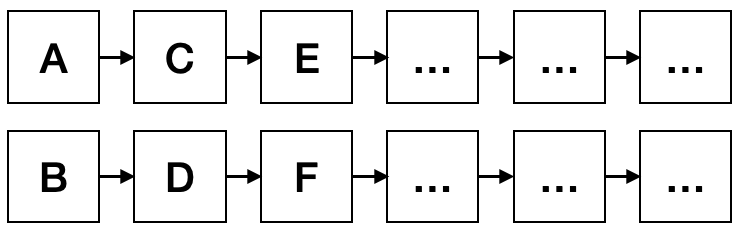
\includegraphics[width=\textwidth]{figure/superscalar.png}
      \caption{2-way superscalar execution.}
      \label{fig:superscalar-2}
  \end{subfigure}
  \caption{Scalar vs. superscalar processor design.}
  \label{fig:superscalar}
\end{figure}

In terms of instruction scheduling, we have in-order scheduling and out-of-order scheduling, or so-called instruction dynamic scheduling. Fig.~\ref{fig:o3} shows the differences between two ways of instruction scheduling mechanism. For example, instruction A requires 3 clock cycles to complete, but instruction B depends on the result of A. In the in-order design, B must wait until A is completed, but in the out-of-order design, we can execute instruction D (that is independent of A) prior to B, so that the performance is further improved. Most of modern processors for high-performance computing are based on out-of-order scheduling design.

\begin{figure}
    \centering
    \begin{subfigure}{0.4\textwidth}
        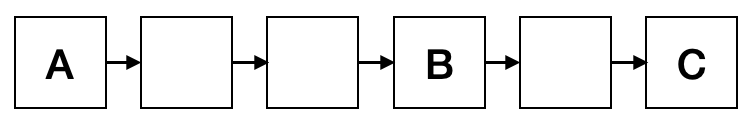
\includegraphics[width=\textwidth]{figure/in-order.png}
        \caption{In-order scheduling.}
        \label{fig:o3-1}
    \end{subfigure}
    ~
    \begin{subfigure}{0.4\textwidth}
        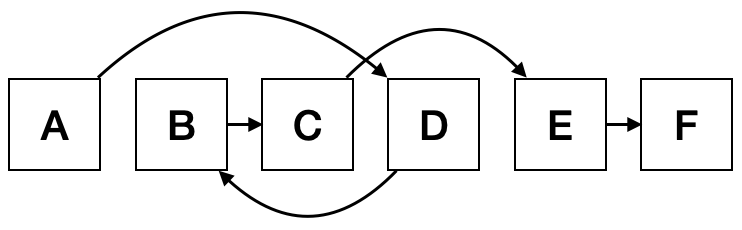
\includegraphics[width=\textwidth]{figure/out-of-order.png}
        \caption{Out-of-order scheduling.}
        \label{fig:o3-2}
    \end{subfigure}
    \caption{In-order vs. out-of-order instruction scheduling mechanism.}
    \label{fig:o3}
\end{figure}

\section{Verification \& SoC Integration} %yyc
% citation will be considered later
% citation: https://www.sciencedirect.com/topics/computer-science/design-verification

% citation: https://www.veripool.org/ftp/verilator_doc.pdf

% citation: https://github.com/riscv/riscv-isa-sim
\subsection{Verification}
The aim of verification is to make sure that the design meets the system requirements and specification. Normal approaches to verify design include following three ways [cite]:
\begin{enumerate}
    \item \textbf{Logic simulation}. The design is verified by performing a cycle accurate simulation. The detailed timing and functionality information can be check to see correctness.
    \item \textbf{Functional verification}. The design is checked against a functional models, which describe the correct behavior of the design. A behavior level simulation is performed to check the correctness of the design while timing detailed are ignored.
    \item \textbf{Formal verification}. This method includes property checking and equivalence checking.
\end{enumerate}

We emphasize on doing functional verification as well as logic simulation. We cannot perform formal verification because normally this requires commercial software support. Due to our budget constraints, we do not use this to check our model. For the logic simulation part, the verification process will be based on the logs and waveform, i.e., we check the logs and waveform to check our design's timing and behaviors. Although by logic simulation we can know whether our design is identical to our expectation, but they may not necessarily meet the RISC-V specification. We will use another verified RISC-V simulator as comparison to check the architectural correctness of our processor.

\subsection{SoC Integration}
A single CPU can do few things as it cannot perform IO. It can only run hardwired program from specific locations. Although we are using many tools to do the evaluation, this still make the whole development process inconvenient. We perform a SoC Integration aiming at providing our SoC IO capabilities, making it possible to dynamically loading program and output its computation result to the host machine. 

The SoC will integrate at least some memory devices. The whole simulation system will provide interface for the simulation host machine to communicate and verify the design under test.
